\documentclass[tikz,border=5pt]{standalone}
\usepackage{tikz}
\usepackage{amsmath}
\usetikzlibrary{positioning,arrows.meta}
\definecolor{nebula}{HTML}{6366F1}
\definecolor{spark}{HTML}{14B8A6}
\definecolor{ink}{HTML}{334155}
\begin{document}
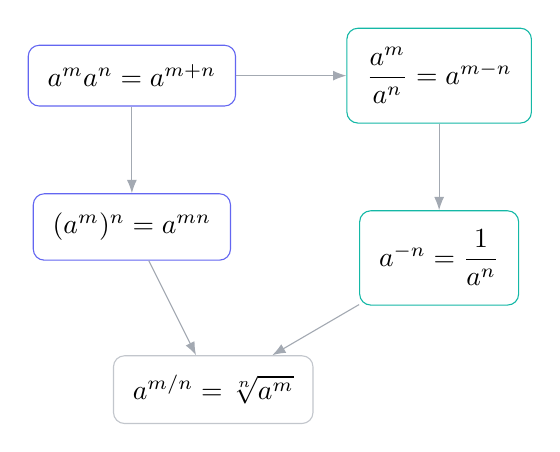
\begin{tikzpicture}[font=\sffamily,>=Latex,node distance=1.1cm and 1.4cm]
  \tikzset{rule/.style={draw=ink!30,rounded corners=4pt,fill=white,inner sep=7pt}}
  \node[rule,draw=nebula] (p) {$a^m a^n=a^{m+n}$};
  \node[rule,right=of p,draw=spark] (q) {$\dfrac{a^m}{a^n}=a^{m-n}$};
  \node[rule,below=of p,draw=nebula] (r) {$(a^m)^n=a^{mn}$};
  \node[rule,below=of q,draw=spark] (s) {$a^{-n}=\dfrac1{a^n}$};
  \node[rule,below right=1.2cm and -1.5cm of r] (t) {$a^{m/n}=\sqrt[n]{a^m}$};
  \draw[->,ink!45] (p)--(q);
  \draw[->,ink!45] (p)--(r);
  \draw[->,ink!45] (q)--(s);
  \draw[->,ink!45] (r)--(t);
  \draw[->,ink!45] (s)--(t);
\end{tikzpicture}
\end{document}
